\documentclass{article}
\usepackage{hyperref,amsmath,amssymb}
\usepackage{tikz,comment}
\usetikzlibrary{automata, arrows.meta, positioning,decorations.pathmorphing}

\begin{document}

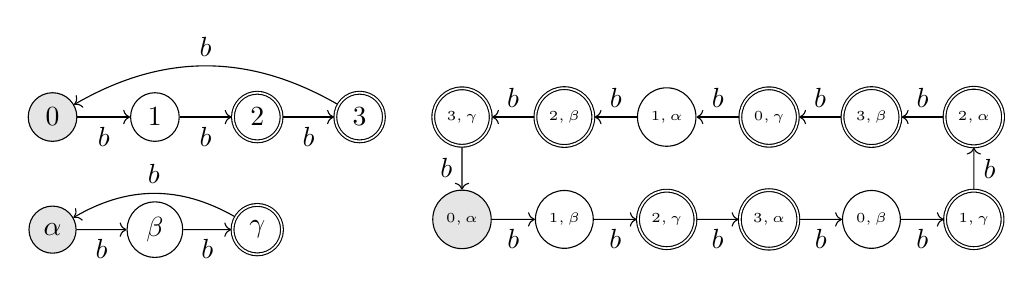
\begin{tikzpicture}[scale=.65]
	\node[draw,circle,fill=black!10] (s0) at (0,0) {$0$};
	\node[draw,circle] (s1) at (2,0) {$1$};
	\node[draw,circle,accepting] (s2) at (4,0) {$2$};
	\node[draw,circle,accepting] (s3) at (6,0) {$3$};
	
	\draw[->] (s0) -- node[below]{$b$} (s1);
	\draw[->] (s1) -- node[below]{$b$} (s2);
	\draw[->] (s2) -- node[below]{$b$} (s3);
	\draw[->] (s3) edge[bend right=30] node[above]{$b$} (s0);
	
	\node[draw,circle,fill=black!10] (t0) at (0,-2.2) {$\alpha$};
	\node[draw,circle] (t1) at (2,-2.2) {$\beta$};
	\node[draw,circle,accepting] (t2) at (4,-2.2) {$\gamma$};
	
	\draw[->] (t0) -- node[below]{$b$} (t1);
	\draw[->] (t1) -- node[below]{$b$} (t2);
	\draw[->] (t2) edge[bend right=30] node[above]{$b$} (t0);
	
	\node[draw,circle,fill=black!10] (p00) at (8,-2) {\tiny $0,\alpha$};
	\node[draw,circle] (p11) at (10,-2) {\tiny$1,\beta$};
	\node[draw,circle,accepting] (p22) at (12,-2) {\tiny$2,\gamma$};
	\node[draw,circle,accepting] (p30) at (14,-2) {\tiny$3,\alpha$};
	\node[draw,circle] (p01) at (16,-2) {\tiny$0,\beta$};
	\node[draw,circle,accepting] (p12) at (18,-2) {\tiny$1,\gamma$};
	
	\node[draw,circle,accepting] (p32) at (8,0) {\tiny $3,\gamma$};
	\node[draw,circle,accepting] (p21) at (10,0) {\tiny$2,\beta$};
	\node[draw,circle] (p10) at (12,0) {\tiny$1,\alpha$};
	\node[draw,circle,accepting] (p02) at (14,0) {\tiny$0,\gamma$};
	\node[draw,circle,accepting] (p31) at (16,0) {\tiny$3,\beta$};
	\node[draw,circle,accepting] (p20) at (18,0) {\tiny$2,\alpha$};

	\draw[->] (p00) -- node[below]{$b$} (p11);
	\draw[->] (p11) -- node[below]{$b$} (p22);
	\draw[->] (p22) -- node[below]{$b$} (p30);
	\draw[->] (p30) -- node[below]{$b$} (p01);
	\draw[->] (p01) -- node[below]{$b$} (p12);
	\draw[->] (p12) -- node[right]{$b$} (p20);
	
	\draw[->] (p20) -- node[above]{$b$} (p31);
	\draw[->] (p31) -- node[above]{$b$} (p02);
	\draw[->] (p02) -- node[above]{$b$} (p10);
	\draw[->] (p10) -- node[above]{$b$} (p21);
	\draw[->] (p21) -- node[above]{$b$} (p32);
	\draw[->] (p32) -- node[left]{$b$} (p00);
\end{tikzpicture}

\end{document}